\section{Improve after deployment}
%[related work]

%An Unsupervised Approach to User Simulation: toward Self-Improving Dialog Systems
%Learning from Dialogue after Deployment - Feed Yourself Chatbot


We propose a framework in this section to discuss the possibility of improving a frame tracking model after its deployment. A deployed dialogue system has the chance of processing through a large number of real dialogues. It would be a huge advantage if we can make use of those data to improve the system. A similar idea is discussed in \cite{hancock2019learning}, where the authors proposed a self-feeding chit-chat dialogue system.
%why? more data, better model
% lifelong learning (Silver et al., 2013) and never-ending (language) learning (Carlson et al., 2010)
In a chit-chat dialogue system, the roles of the user and the system are symmetric. This is not true for a goal-oriented dialogue system, so we adapt their method to fit into our setting.
% (Similar strategy may be used for improving NLU.)

The main idea is to obtain user feedback as frame tracking labels of the corresponding dialogues.
%how to collect user feedback without too much extra effort of a normal user. simple and user-friendly, user experience
There are many ways to achieve this. Here we design a framework that collects active user-feedback while still being user friendly and taking care of user experience.
Due to the time constraint of this project, we don't implement and experiment with this framework.

\subsection{Proposed framework}
%detect low user satisfaction, which means that the system made a mistake in the previous turn
Our system asks for feedback only when the estimated user satisfaction is low, in other words, when it thinks it made a mistake (in the previous turn). Comparing to asking for feedback at every turn, this should reduce the extra effort imposed on a normal user of the system.
% active learning, detect mistake Hashimoto and Sassano (2018)
%ask for correction (in a smart, helpful manner), use the correction from user as feedback labels.
When asking for feedback, the system provides a guess at the same time to be helpful and offer a better user experience. The user feedback is then transformed into training data and labels.

%[example dialogues showing how the system works]

Ideally, in the context of frame tracking, the user feedback would tell us the correct frame reference. This is however infeasible because the concept of frame reference is too complicated to incorporate into a normal dialogue. Instead, correcting or confirming a slot value is more reasonable in terms of the amount of work imposed on the user. So when asking for feedback, the system would pick a slot in the previous turn and ask for correction. This operation is better to be done using natural language rather than an abrupt multiple choice question or a list of options so that the data collection part and the original dialogue are seamlessly combined.

% how to use the feedback: transform user feedback into frame tracking data, and use a multitasking model
This system consists of three tasks. The first one is the frame tracking task.
% satisfaction task
The second one is the satisfaction task, which is used to decide when to ask for feedback. The input of the satisfaction task is the user utterance and the output is a binary class indicating whether the system should ask for feedback or not.
%[write more?]
% feedback task
The last and most important one is the feedback task. The label we have for this task is a slot value in the referred frame, so this is the target we want to predict rather than the frame reference itself as in frame tracking task. However, we still want to make it as similar to frame tracking as possible so that the system can improve on frame tracking when training on feedback data. To account for this, we define the feedback task as follows. The input consists of two parts: the same input as of frame tracking, i.e.\ NLU labels of the current utterance and a list of frames, and the other part is a candidate slot value. The goal of this task is to predict whether the candidate slot value is a correct one, in other words, whether this slot value appears in the referred frame.
% We heavily rely on the assumption that ... slot value <-> frame reference

Inspired by \cite{hancock2019learning}, we propose to combine these three tasks using multitask learning, hoping that training on new feedback data gathered after deployment would improve the performance of frame tracking. Figure \ref{fig:multitask} is an example of a multitask learning model.

%[example of model architecture]
\begin{figure}
    \centering
    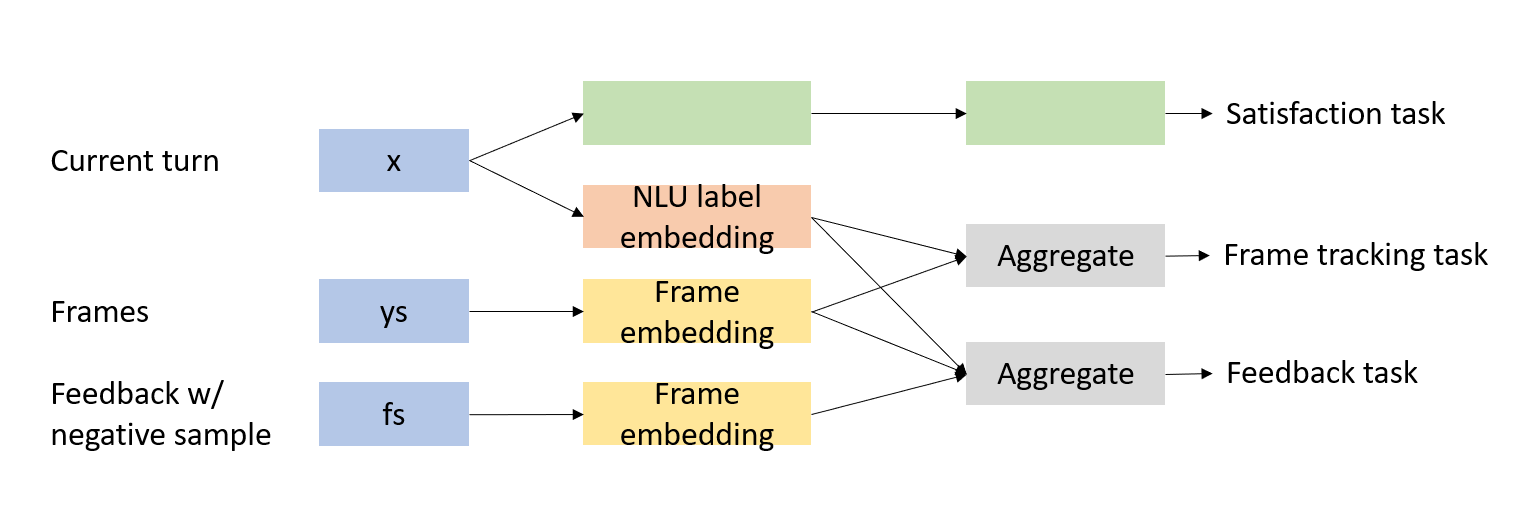
\includegraphics[width=\columnwidth]{figures/multitask2.png}
    \caption[An example of frame tracking after deployment]{Example model for frame tracking after deployment.}
    \label{fig:multitask}
\end{figure}

% the procedure of the pipeline, as a summary
Here we give a procedure of how to create the whole system from scratch.
\begin{enumerate}
    \item Train on Frame tracking task
    \item Collect data for Satisfaction task
    \item Train on Frame tracking + Satisfaction
    \item Deploy and collect data for Feedback task
    \item Train on Frame tracking + Satisfaction + Feedback
    \item Back to step 4.
\end{enumerate}
